\documentclass[10pt]{article}
\usepackage{amsmath,amssymb}
\setlength{\oddsidemargin}{0in}
\setlength{\evensidemargin}{0in}
\setlength{\textheight}{9in}
\setlength{\textwidth}{6.5in}
\setlength{\topmargin}{-0.5in}
\usepackage{enumitem}
\usepackage{graphicx}
\usepackage{float}
\DeclareMathOperator*{\argmax}{arg\,max}
\DeclareMathOperator*{\argmin}{arg\,min}
\title{\bf Math 170S\@: Homework 6}
\date{11/21/2023}
\author{\bf Owen Jones}

\begin{document}
\maketitle
\begin{enumerate}[label=\textbf{Problem \arabic*.}]
    \item \begin{itemize}
        \item [1.] $H_0:\mu=3.4$ liters.
        \item [2.] $H_1:\mu>3.4$ liters.
        \item [3.] Let $T:=\frac{\overline{x}-\mu}{\frac{s}{3}}\sim t^{(8)}$
        \item [4.] Graph below shows t distribution with $8$ degrees of freedom. Shaded region descibes $C:=\{\overline{x}|\overline{x}>3.5033\}$
        %$P(\overline{x}>\mu+t^{(8)}_{0.05}\frac{s_x}{3}|H_0)\Leftrightarrow P(T>t^{(8)}_{0.05}|H_0)=0.05$ or
        \begin{figure}[H]
            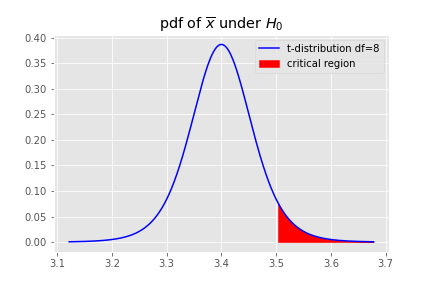
\includegraphics[scale=0.5]{170S_hw_6_Q_1.png}
        \end{figure}
        \item [5.] $\displaystyle\overline{x}=\frac{1}{9}\sum_{i=1}^{9}x_i=3.55,s_x=\sqrt{\frac{\displaystyle\sum_{i=1}^{9}{(x_i-\overline{x})}^2}{8}}=0.167\Rightarrow T=\frac{\overline{x}-\mu}{\frac{s_x}{3}}=2.80$
        \item [6.] We choose to reject the null in favor of the alternative hyppothesis.
        \item [7.] $p-value=P(\overline{x}>3.55|H_0)=0.0115<0.05$
    \end{itemize}
    \item Let $Z:=\frac{Y-np}{\sqrt{np(1-p)}}=\frac{Y-0.08\cdot 100}{\sqrt{100\cdot 0.08(1-0.08)}}\approx\mathcal{N}(0,1)$ by CLT.\\
    Let $z_\alpha:=|\frac{6-0.08\cdot 100}{\sqrt{100\cdot 0.08(1-0.08)}}|$. Want to find $\alpha$ s.t $P(Z<-z_\alpha)=\alpha$. $z_\alpha=0.737\Rightarrow \alpha=0.230$\\
    Without normal approximation $\displaystyle P(Y\le 6|p=0.08)=\sum_{k=0}^{6}\begin{pmatrix}    100\\   k\end{pmatrix}0.08^k0.92^{100-k}=0.3032\Rightarrow \alpha=0.3032$
    \item \begin{itemize}
        \item [1.] Let $Z:=\frac{Y-np}{\sqrt{np(1-p)}}=\frac{Y-0.75\cdot 192}{\sqrt{192\cdot 0.75(1-0.75)}}\approx\mathcal{N}(0,1)$ by CLT.\\
        Let $z_\alpha:=\frac{152-0.75\cdot 192}{\sqrt{192\cdot 0.75(1-0.75)}}=1.33$.
        $\alpha=P(Y\ge 152|p=0.75)\approx P(Z>z_\alpha)=0.091$
        \item [2.] Let $Z:=\frac{Y-np}{\sqrt{np(1-p)}}=\frac{Y-0.08\cdot 192}{\sqrt{192\cdot 0.08(1-0.08)}}\approx\mathcal{N}(0,1)$ by CLT.\\
        Let $z_\beta:=\frac{152-0.08\cdot 192}{\sqrt{192\cdot 0.08(1-0.08)}}=36.34$.
        $\beta=P(Y<152|p=0.08)\approx P(Z<z_\beta)=1$
    \end{itemize}
    \item We choose $H_0:m=0$ and $H_1:m>0$\\
    Let $\displaystyle W:=\sum_{i=1}^{15}[sgn(X_i-Y_i)]R_i=54$\\
    Let $Z:=\frac{W}{\sqrt{\frac{n(n+1)(2n+1)}{6}}}\approx \mathcal{N}(0,1)$\\
    $P(W\ge 54|H_0)\Leftrightarrow P(Z\ge \frac{54}{\sqrt{\frac{15(16)(31)}{6}}}|H_0)=0.0625$, so we would fail to reject $H_0$ at an $\alpha=0.05$.
\end{enumerate}
\end{document}